\documentclass{article}
\usepackage{tikz}
\usetikzlibrary{arrows, shapes, positioning}
%\tikzstyle{nodeobserved} = [circle, minimum size = 10mm, thick, draw =black!80]
\usetikzlibrary{external}
\tikzexternalize


\begin{document}

\begin{figure}
    \centering
    \tikzsetnextfilename{dag-preds}
    \begin{tikzpicture}
        \node (z1) at (-1,1) {$z_1$};
        \node (z2) at (0,1) {$z_2$};
        \node (z3) at (0,2) {$z_3$};
        \node (w) at (1,1) {$w$};
        \node (u) at (.75,.25) {$u$};
        \node (y) at (-0.5,0) {$y$};
        \node (v) at (-0.5,-1) {$v$};

          \path[->] (z1) edge (y)
                    (z3) edge (z2)
                    (u) edge (z2)
                        edge (y)
                    (z2) edge (w)
                         edge (y)
                     (y) edge (v);
    \end{tikzpicture}
\end{figure}


\begin{figure}
    \centering

    \tikzsetnextfilename{dag-bmi}
    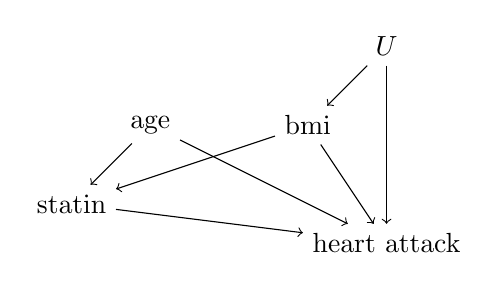
\begin{tikzpicture}
      % Nodes
      \node (bmi) at (1, 1) {bmi};
      \node (age) at (-1, 1) {age};
      \node (u) at (2, 2) {$U$};
      \node (t) at (-2, 0) {statin};
      \node (y) at (2, -0.5) {heart attack};

      % Edges
      \draw[->] (u) -- (bmi);
      \draw[->] (u) -- (y);
      \draw[->] (age) -- (t);
      \draw[->] (bmi) -- (t);
      \draw[->] (age) -- (y);
      \draw[->] (bmi) -- (y);
      \draw[->] (t) -- (y);

    \end{tikzpicture}

\end{figure}

\begin{figure}
    \centering

    \tikzsetnextfilename{policy}
    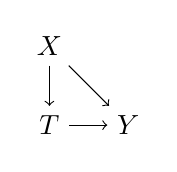
\begin{tikzpicture}
      % Nodes
      \node (x) at (-1, 1) {$X$};
      %\node (z) at (0,  1) {$Z$};
      \node (t) at (-1, 0) {$T$};
      \node (y) at (0,  0) {$Y$};

      % Edges
      \path[->] (x) edge (t)
                    edge (y)
                %(z) edge (t)
                    %edge (y)
                (t) edge (y);

    \end{tikzpicture}
    
\end{figure}



\end{document}
